\section{Case Study: Real-time feedback control of a hexrotor with contract based estimation and robust control}
\label{sec:experiments}

\subsection{Experimental setup}
To evaluate our methodology on a real platform, we applied it to a hexrotor with the Odroid U3 as a computation platform and running the Robot Operating System (ROS) in Ubuntu. For the evaluation, the hexrotor is tasked with repeatedly following a given circular trajectory.
As can be seen in Fig.~\ref{fig:time_ecdf}, the visual odometry algorithm can occcasionaly take a long time to get a pose estimate. In our formulation in section \ref{robustMPC} we have assumed that the estimator satisfies the $(\delta, \epsilon)$ contract requested by the controller. Thus, to ensure that the estimator fulfills the contract and the mathematical guarantees that our RAMPC formulation provides hold, instead of using the visual odometry algorithm to fly the robot, we injected delays and errors into the measurements from the Vicon system. These delays and errors were selected from the $(\delta,\epsilon)$ curve obtained by profiling the SVO algorithm (see Section \ref{sec:visual_odometry}).
The hexrotor flies using these pose estimates and our Robust Model Predictive Algorithm for both the position control of the hexrotor and setting the time deadline for the next estimate. The RAMPC, is coded in CVXGEN \cite{} and the generated C-Code is integrated in the ROS module for position control of the hexrotor. The set computations for the feasible sets are done offline in MATLAB and then used in CVXGEN as Polyhedron type constraints ($Hx \le g$). 
%For the contract based perception and estimation algorithm we use the FAST corner detector (as in section \ref{}) providing measurements to an Unscented Kalman Filter that also uses measurements from an Inertial Measurement Unit (IMU) to provide a state estimate for the control algorithm to use.
Later in this section we show how our approach dynamically schedules different modes of the contract-based perception and estimation algorithm at run-time and also controls the dynamic system in an energy-efficient way while providing good tracking performance. In the evaluation subsection we will compare our results to a baseline Model Predictive Control algorithm that does not leverage co-design and operates at fixed ($\delta,\epsilon$) points of the perception/estimation algorithm which provides a state estimate to the controller.

\todo[author=KM,inline]{Do we want an architecture diagram of the way the hexrotor is controlled using ROS?}
\todo[author=YVP,inline]{Yes, the trajectory generator to MPC/RAMPC to low level part would be good to show and make for a nice fig.}
%The control performance, as measured by a function that factors in the error in following the flight path and the cost of control, is shown in Fig.~\ref{fig:CostAndModes}.
%(The details of this cost function are given in Section \ref{formulation}).


\subsection{Profiling the perception and estimation pipeline}

Recall that in section \ref{robustMPC}, the control algorithm needs the profiled ($\delta,\epsilon$) curve for the perception and estimation algorithm. In our experimental setup, we need the performance of the SVO algorithm to formulate the RAMPC for control of the hexrotor. Figure \ref{fig:svo_error_delay} shows the bound on estimation error and the $90^{th}$ percentile execution times for a different number of maximum corners in the SVO algorithm through extensive flying over a relatively feature-rich environment (Figure \ref{fig:nanohex}). The estimation error is computed with the help of ground truth obtained through the Vicon motion capture system. We profiled the performance for the same trajectory with different settings of the odometry offline by logging images and IMU data in-flight, and then running the visual odometry code on the Odroid-U3 offline.
This accurately recreates the in-flight environment that is present for the visual odometry algorithm and this profiling is then used online for making in-flight decisions by the control algorithm.

Also needed for the control optimization as stated in equation \ref{eq:tractableOptim} is a measure of the power consumption by the visual odometry while at different settings on maximum number of corner. This is obtained again by running the visual odometry code offline for different knob settings and measuring the power consumed by the Odroid to perform these computations. Power measurements are made using the Odroid Smart Power meter \cite{OdroidSmartPower}, which measures consumption at 10Hz to milliwatt precision. We measure the power consumption of the entire Odroid board, including CPU and DRAM power consumption. To avoid the physical challenges of fitting the power meter onto our hexrotor platform, we measure the power consumption of the Odroid board on the ground, running the same controller and vision workloads as it does during flight as explained above. Since the profiling of power is done offline with other peripherals plugged into the odroid (e.g. A monitor and keyboard), we measure the idle power of the Odroid and subtract that from the power measurements when the SVO algorithm is running on it in different modes. This gives us a more accurate measure of the workload the visual odometry task is responsible for. This offline profiling now allows us to formulate the co-design problem for the hexrotor and experimentally evaluate our methods.


\begin{figure}[htbp]
  \centering
  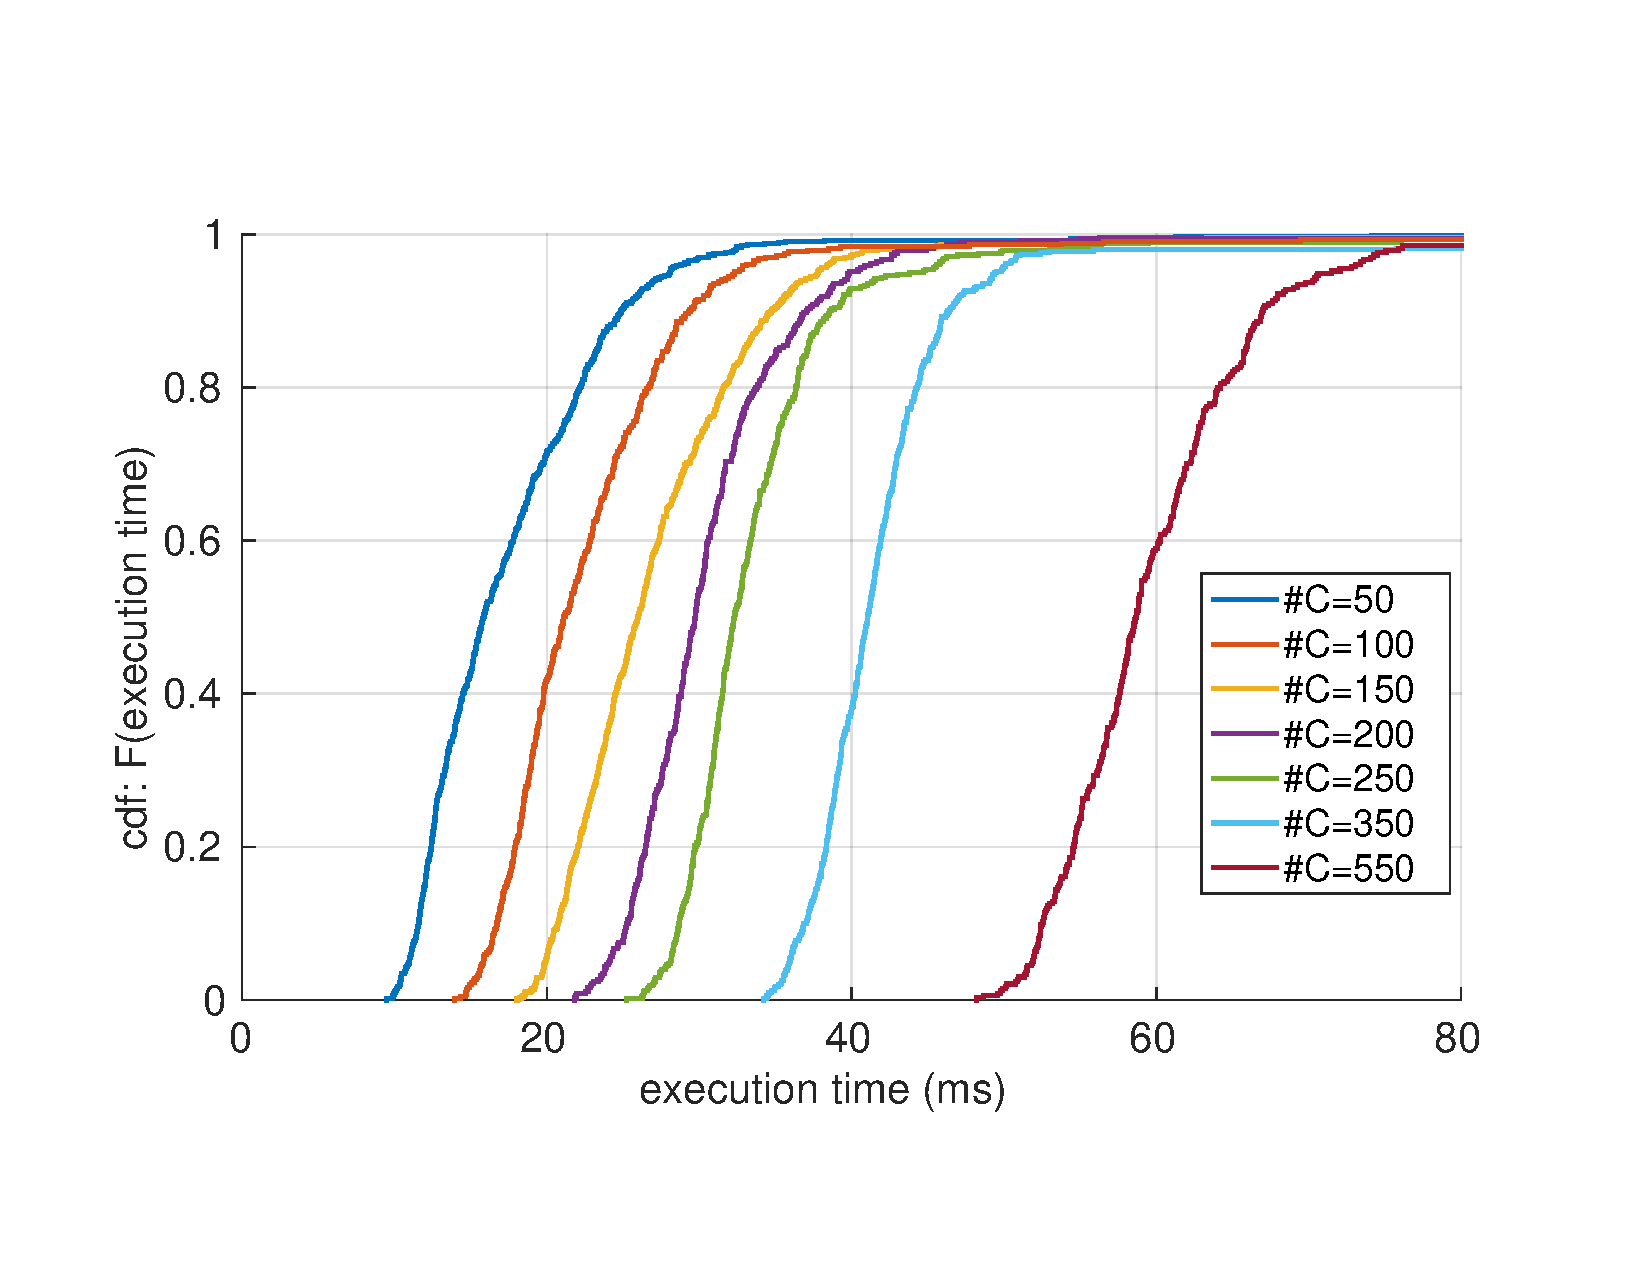
\includegraphics[width=0.9\columnwidth]{figures/time_ecdf_millisec.pdf}
  \caption{Cumulative distribution of profiled execution times for visual odometry running on the Odroid-U3 for varying maximum number of corners from the SVO algorithm.}
  \label{fig:time_ecdf}
\end{figure}



\subsection{Experimental Evaluation}

After profiling the performance of the perception and estimation algorithm and formulating the Robust MPC controller for the hex-rotor model (equation \ref{}), we experimentally evaluate the tracking performance and estimated energy consumption based on actual flights around a pre-defind trajectory. For comparision, we use a Model Predictive Controller with the same cost function and initial feasible sets as in our Robust MPC formulation. Comparision to such a controller would give a baseline to measure the benefits of our co-design method against the a similar control algorithm that does not leverage co-design and is unaware of the estimator algorithm that gives it a state estimate. 

For the evaluation, we fly in a predefined trajectory as shown in figure \ref{}, repeating the experiment 10 times to gather enough data to conclusively measure the performance of Robust MPC and MPC with fixed modes of ($\delta,\epsilon$). Note that since the controller was a sampled discrete-time controller working with simulated 20Hz camera updates, this realistically restricts us to using modes of estimator operation with delay ($\delta$) less than (1/20s), or one sampling period, i.e. modes corresponding to 50, 100, 150 and 200 maximum corners from the FAST detector (see figure \ref{fig:svo_error_delay}). These modes and their estimated power consumption is in table \ref{tbl:modes_exp}. Note, \#C represents maximum number of FAST corners requested, $\epsilon$ shows the worst case error bound on the state estimate, $\delta$ is the $90^{th}$ percentile execution time for that mode, and $P$ represents the expected power consumption in that mode as profiled offline. This power consumption is the computation power used by a particular mode in excess to the idle power for the Odroid used for profiling, which was 1.5W.

\begin{table}[htb]
\begin{center}
\caption{Estimation modes used in the experiment.}
\label{tbl:modes_exp}
\begin{tabular} {|c|c|c|c|c|}
	\hline
	\textbf{Mode} & \textbf{\#C} & $\pmb{\epsilon}$ & $\pmb{\delta}$ \textbf{(ms)} & $\pmb{P}$\textbf{(W)} \\ \hline
	0 & 50 &  24.88 & 0.028 &  0.778  \\ \hline
 	1 & 100 & 29.82 & 0.0237 &  0.862  \\ \hline
	2 & 150 & 34.66 & 0.0230 & 0.870 \\ \hline
	3 & 200 & 38.01 & 0.0113 & 0.951 \\ \hline
	\end{tabular}	
	\end{center}
\end{table}




\subsection{Experimental Results}

Once the flights are complete, to get a more accurate picture of how the controllers really performed, we use the following function to measure tracking performance at each time step.

\begin{equation}
	J_{true}(t) =  (x(t)-x_{ref}(t))^{T}Q(x(t)-x_{ref}(t)) + u(t)^{T}Ru(t)
\end{equation}

Note that since we have access to the true position and velocities ($x(t)$) of the hexrotor with the VICON system, we can obtain the true tracking cost. Table \ref{tbl:RAMPC_MPC_performance} shows the mean of the above function over the 10 flights for both MPC across all fixed modes and RAMPC with different values of $\alpha$. It also shows the estimated energy consumption based on the time spent in each mode (which can be seen in Table \ref{tbl:RAMPC_ModeTime} for RAMPC). RAMPC shows better tracking performance (lower mean $J_{true}$) than the MPC with either of the 4 fixed modes, showing the improved control performance that can be obtained by dynamically switching between estimation modes in-flight at runtime. 

\begin{figure}[tbh]
	\centering
	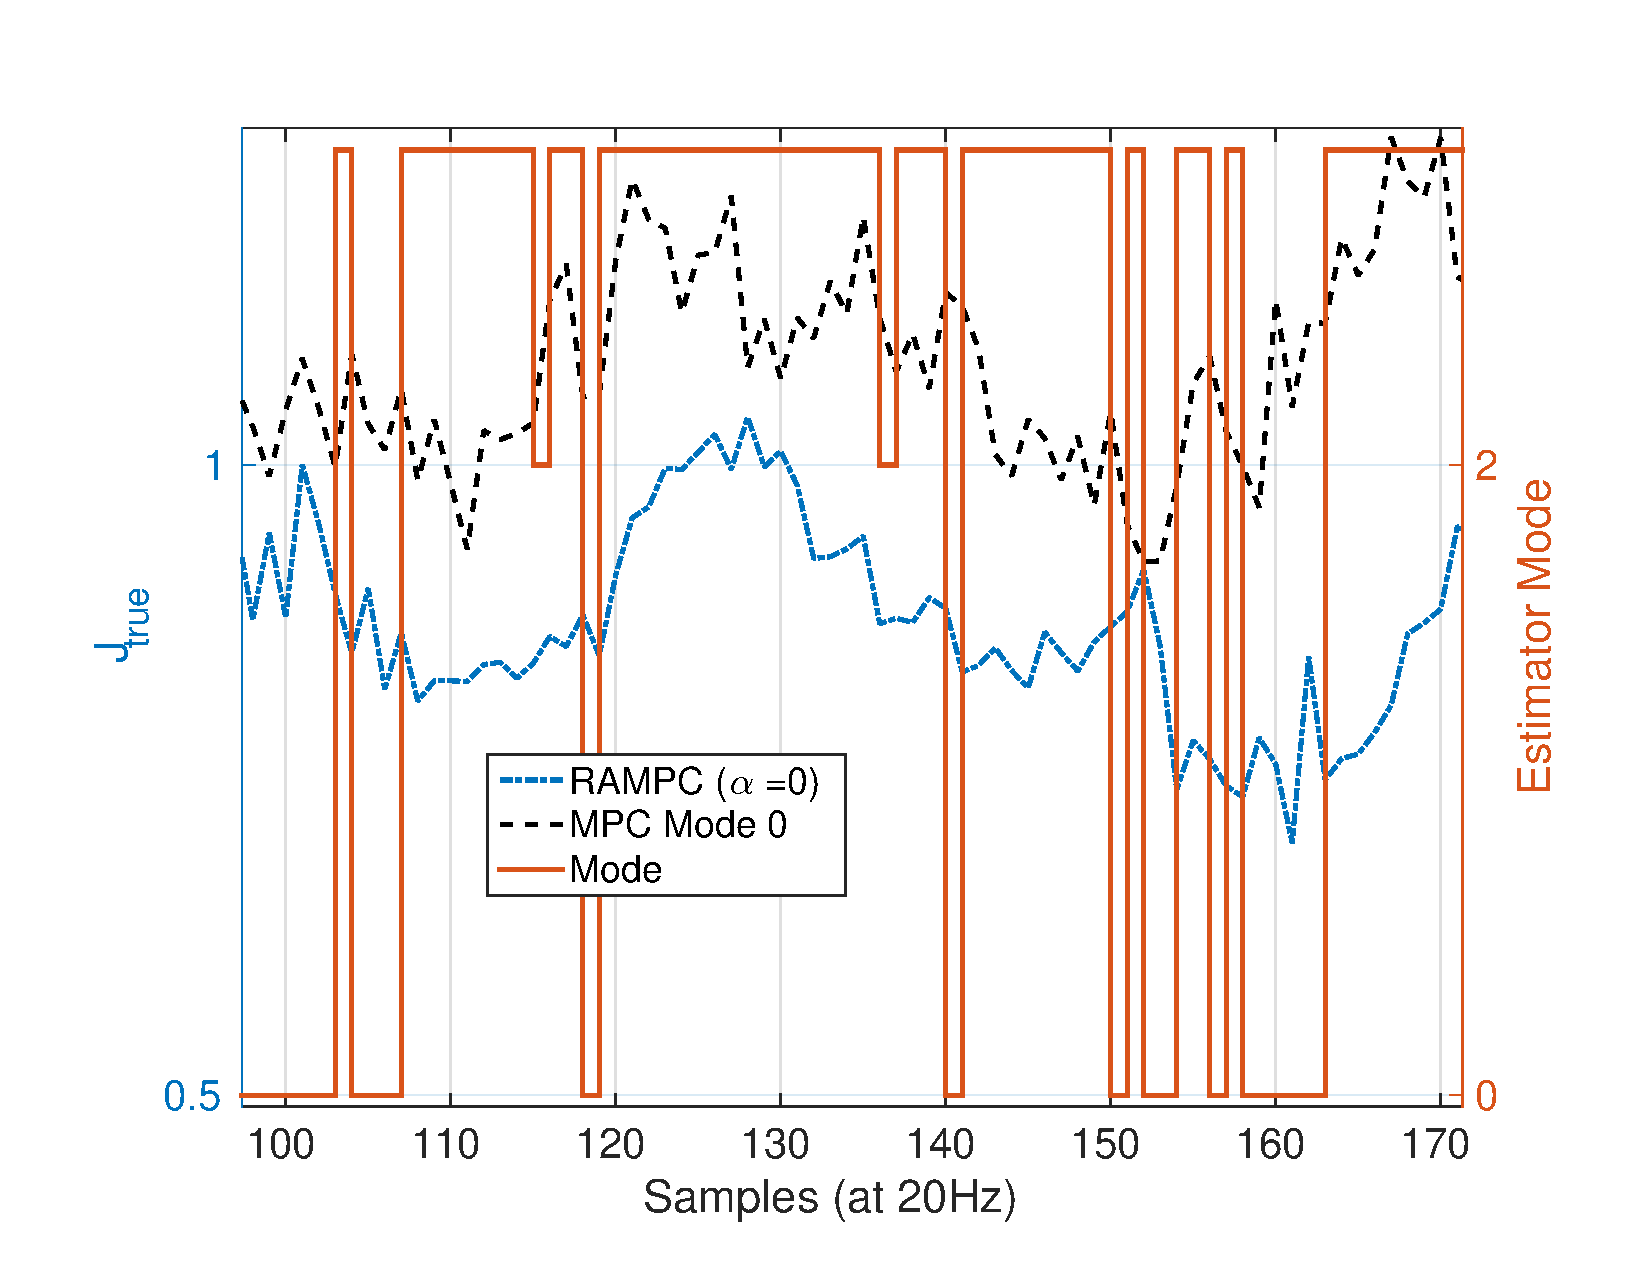
\includegraphics[width=0.49\textwidth]{figures/CostAndModes}
	\caption{Tracking cost at each time step for MPC (fixed mode 0 estimator) and RAMPC with $\alpha=0$. Note how the RAMPC performs better (lower cost) than the MPC and there is dynamic switching of estimator modes at runtime leading to improved performance for the RAMPC.}	
	\label{fig:CostAndModes}
\end{figure}


Figure \ref{fig:CostAndModes} shows how the tracking cost ($J_{true}$) evolves over time for RAMPC (with $\alpha=0$) and MPC (fixed mode 0) for a portion of the hexrotor flight. The estimator modes selected by RAMPC are overlaid in orange. Figure \ref{fig:CostAndModes} demonstrates that RAMPC has uniformly lower tracking cost than MPC, enabled by RAMPC's dynamic switching of estimator modes at runtime. Note that RAMPC exhibits better tracking performance throughout the flight and not just in this portion, and also outperforms MPC at other modes (see Table \ref{tbl:RAMPC_MPC_performance}).

Figure \ref{fig:TrackingVsEnergy} shows that RAMPC provides better tracking performance while using less energy to do so. For any fixed energy budget (a point on the x-axis), RAMPC delivers lower tracking cost (y-axis) than MPC. While MPC's tracking error is relatively constant across modes, RAMPC is able to balance tracking error with energy consumption by varying the $\alpha$ parameter. RAMPC's switching between estimation modes improves not only the control performance but also energy efficiency.


\begin{figure}[tbh]
	\centering
	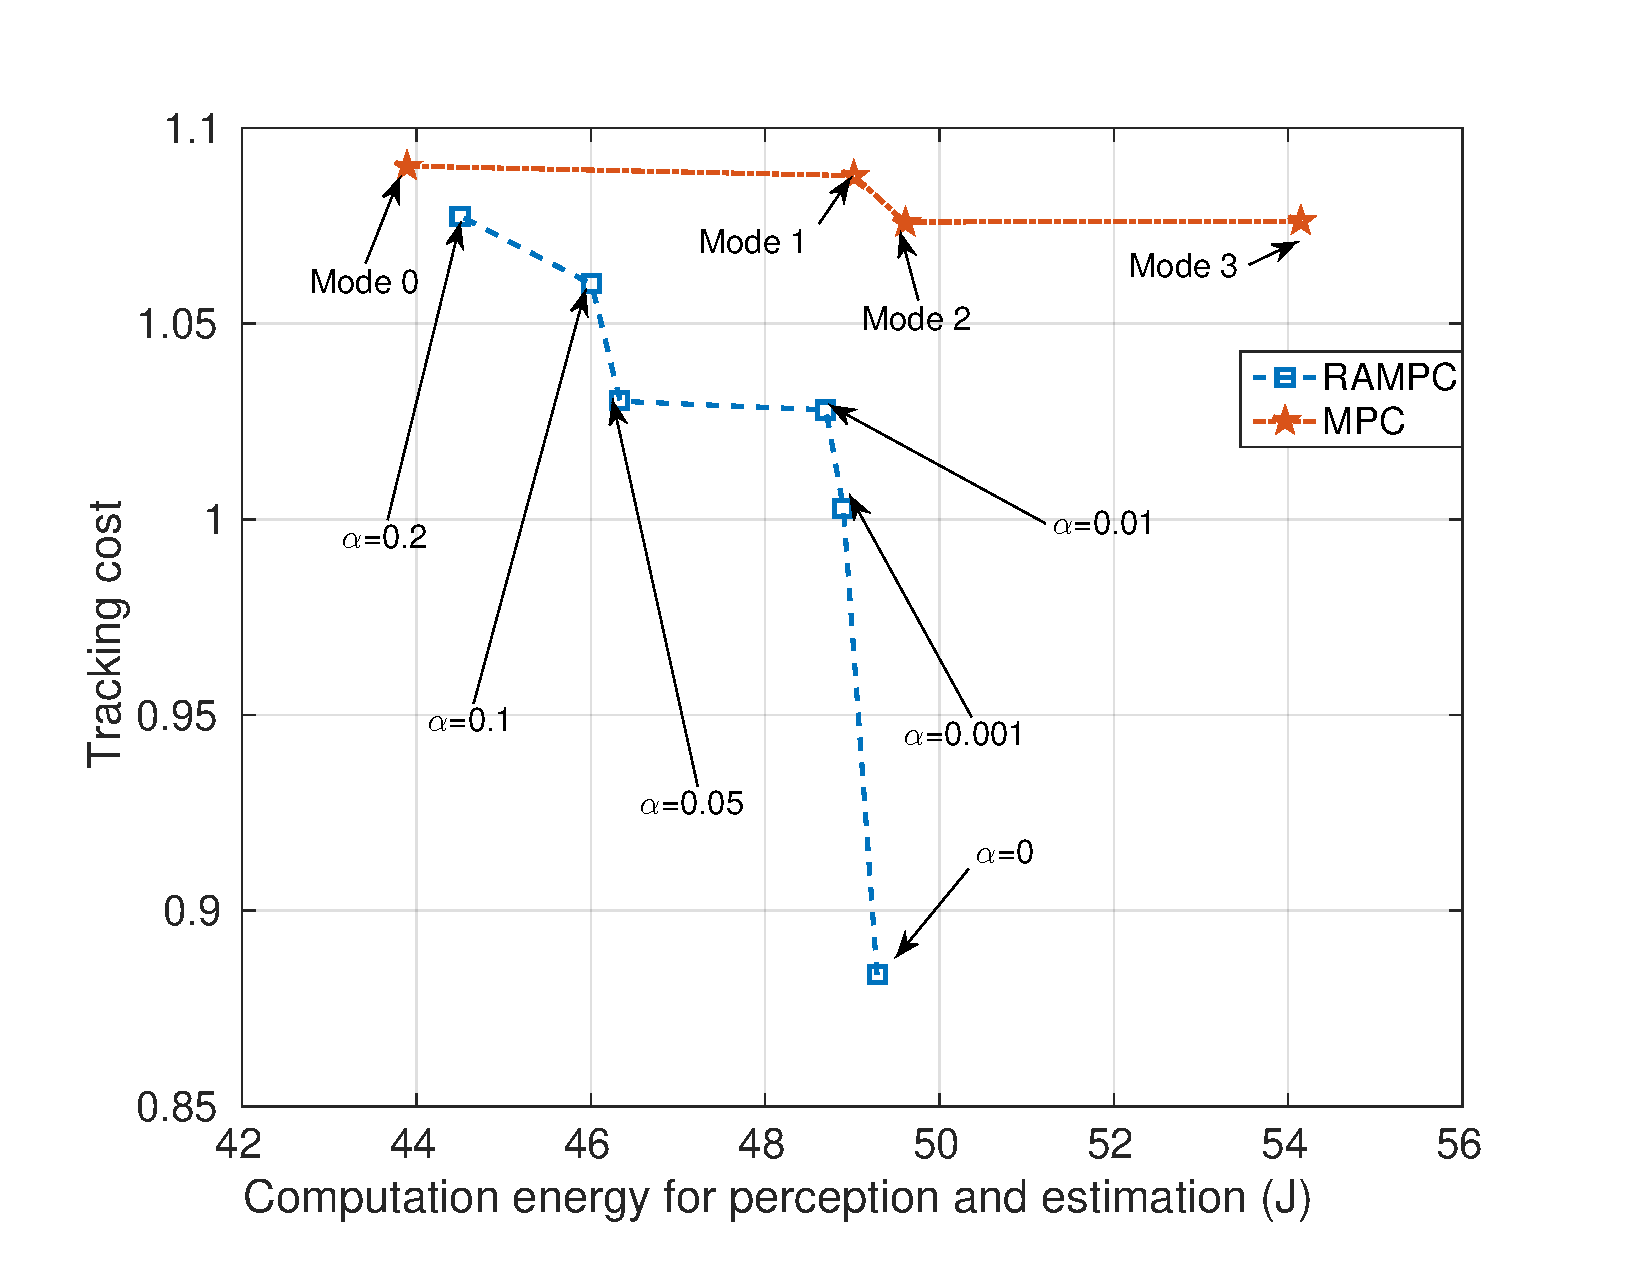
\includegraphics[width=0.49\textwidth]{figures/TrackingVsEnergy}
	\caption{Tracking cost vs estimated computation energy for executing the perception and estimation algorithm. Note for MPC, different energies are realized only by operating at different fixed modes of the perception and estimation algorithm. Using RAMPC as the controller, the different energies are due to run-time scheduling of different modes based on the optimal value of the cost function of Eq. \ref{eq:tractableOptim} at each time step based on different values of $\alpha$. It is worth noting that RAMPC with co-design outperforms standard MPC on tracking performance across the entire range of energy consumption.}
	\label{fig:TrackingVsEnergy}
\end{figure}


\begin{table}[htb]
\begin{center}
\caption{Tracking performance and computation energy}
\label{tbl:RAMPC_MPC_performance}
\begin{tabular} {|c|c|c|c|c|}
	\hline
	\textbf{Controller} &\textbf{Est. Mode}/ $\pmb{\alpha}$ & $\pmb{E[J_{true}]}$ & $\pmb{\sigma({J_{true}})}$ & $\pmb{Energy(J)}$ \\ \hline
	MPC & 0/ $-$ & 1.0903 & 0.104 & 43.89\\ \hline
	MPC & 1/ $-$ & 1.0878 & 0.087 & 49.02 \\ \hline
	MPC & 2/ $-$ & 1.0760 & 0.098 & 49.60 \\ \hline
	MPC & 3/ $-$ & 1.0762 & 0.088 & 54.15 \\ \hline
	RAMPC &  $-$/0 & 0.8836 & 0.079 & 49.28 \\ \hline
	RAMPC & $-$/ 0.001 & 1.0029 & 0.093 & 48.90  \\ \hline
	RAMPC & $-$/ 0.01 & 1.0280 & 0.089 & 48.69  \\ \hline
	RAMPC & $-$/ 0.05 &1.0302 & 0.096 & 46.33 \\ \hline
	RAMPC & $-$/ 0.1 &1.0601 & 0.086 & 46.01 \\ \hline
	RAMPC & $-$/ 0.2 & 1.0776 & 0.083 & 44.49 \\ \hline
\end{tabular}	
	\end{center}
\end{table}



Figure \ref{fig:CostAndEnergyVsAlpha} shows the degradation (increased mean $J_{true}$) in tracking performance and reduction in energy consumption as the weight $\alpha$ for the computation power consumption in the cost function is increased. As energy becomes more important, RAMPC smoothly balances tracking cost and energy consumption. Table \ref{tbl:RAMPC_ModeTime} quantifies how RAMPC makes this trade-off, by showing the fraction of time spent in the 4 modes with RAMPC as $\alpha$ changes. While time is split between modes 0 and 3 with $\alpha=0$, more and more time is spent in the low-power (but less accurate) mode 0 as $\alpha$ increases.


\begin{figure}[t]
	\centering
	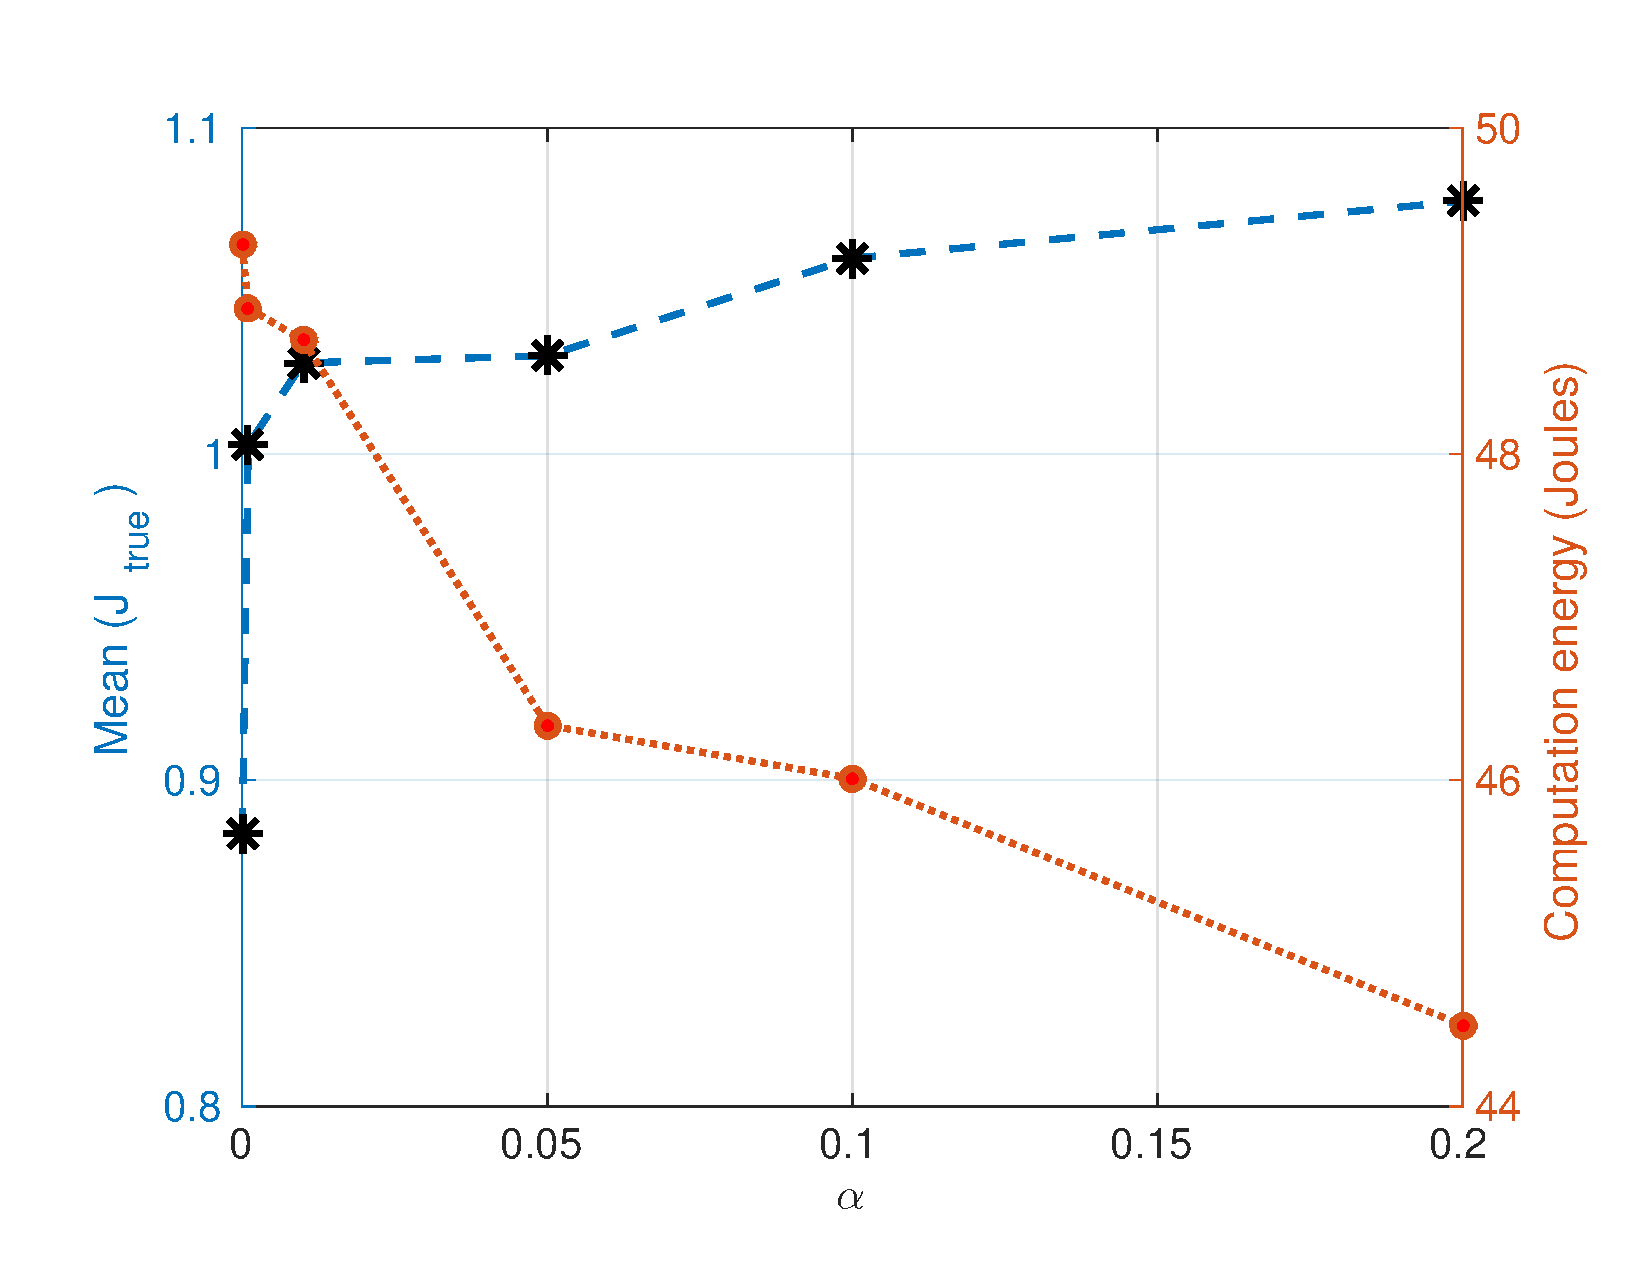
\includegraphics[width=0.49\textwidth,scale=0.7]{figures/CostAndEnergyVsAlpha}
        \vspace{-20pt}
	\caption{RAMPC tracking cost and estimated computation energy for the perception and estimation algorithm as a function of $\alpha$. }
	\label{fig:CostAndEnergyVsAlpha}
\end{figure}


\begin{table}[htb]
\begin{center}
\caption{Fraction of time spent in different estimator modes as $\alpha$ changes for RAMPC}
\label{tbl:RAMPC_ModeTime}
\begin{tabular} {|c|c|c|c|c|}
	\hline
	$\pmb{\alpha}$ & \textbf{Mode 0} & \textbf{Mode 1} & \textbf{Mode 2} & \textbf{Mode 3} \\ \hline
	0 & 0.461 & 0.009 & 0.020 & 0.510 \\ \hline
 	0.001 &  0.494 & 0.001 & 0.029 & 0.467 \\ \hline
	0.01 & 0.512 & 0.005 & 0.039 & 0.444  \\ \hline
	0.005 &  0.692 & 0.000 & 0.156 & 0.152 \\ \hline
	0.1 & 0.691 & 0.000 & 0.218 & 0.091 \\ \hline
	0.2 & 0.897 & 0.000 & 0.098 & 0.005  \\ \hline
	\end{tabular}	
	\end{center}
\end{table}


